Quanten Computing ist eine relativ junge Disziplin der Physik und Informatik. Während sich die beiden Bereiche unabhängig von einader Anfang des 20. Jahrhundert entwickelt hatten, wurden die ersten Versuche und theoretischen Überlegungen, Methoden der Informatik mithilfe von Quantenobjekten umzusetzen um 1980 gestartet. Obwohl das Quantencomputer erst seit kurzer Zeit existiert, hat es bereits bedeutende Fortschritte gemacht und besitzt ein enormes Potenzial für Entwicklungen zum Beispiel in den Bereichen Kryptographie, Optimierungsprobleme, Simulation chemischer Prozesse und maschinelles Lernen.

\subsection{Ein theoretischer Quantencomputer}
Ein der Informatik zugrunde liegendes Prinzip ist, dass \cite[S122]{steane_quantum_1998} Informationen auf unterschiedlichen Weisen dargestellt (codiert) werden können. So kann die Zahl \textit{fünf} zum Beispiel binär ($0101$) oder als Unicode Zeichen (\textit{U+0035}) dargestellt werden. Der Inhalt der Information ist in beiden Fällen jedoch der gleiche.\\
Dieses Prinzip ist für die Informatik sehr wichtig. Es ermöglicht Maschinen komplexe Informationen zu speichern, mithilfe einfacher Operationen zu manipulieren und wieder in ein komplexes Format zu überführen ohne dabei an Informationsgehalt zu verlieren oder Informationen unkenntlich zu zu machen. In einem Computer werden diese Informationen in Form von \textit{bits} darstellt die zwei Zustände, repräsentiert durch \textit{0} und \textit{1}, annehmen können. In einem klassischen, digitalen Computer sind diese beispielsweise durch das fließen von Strom abgebildet. Ein Quantencomputer repräsentiert Informationen in den Eigenschaften von Quanten-Objekten, beispielsweise dem Spin von Elektronen.\\
%% Universaler Quantencomputer ???
Um die Funktion eines Quantencomputer zu erläutern muss erst ein kurzer Blick auf einige Quantenphysikalische Phänomene geworfen werden.

\subsubsection{Superpositionen}
Eine Superposition ist das Fundamentale quantenphysische Phänomen das einem Quantencomputer zugrunde Liegt.
Es wird meistens mithilfe des Gedankenexperiments von \cite[\$5]{schrodinger_gegenwartige_1935} \textit{Schrödingers Katze} veranschaulicht: In einer Box befindet sich eine Katze und ein Gefäß mit Gift das zerstört wird und die Katze tötet wenn ein radioaktiver Zerfall gemessen wird. Von außerhalb der Box lässt sich nicht feststellen ob der Mechanismus der das Gift freisetzt aktiviert wurde. Sie befindet sich, Quantenmechanisch gesehen, in einem Zustand in dem sie sowohl Tot als auch lebendig ist. In dem Moment in dem die Box geöffnet wird, kann festgestellt werden welcher der beiden Zustände eingetroffen ist.\\
Auf ein Quantenteilchen übertragen heißt das: Es kann sich in einem Undefinierten Zustand befinden, der \textbf{Superposition} aus allen möglichen Zuständen. Erst wenn \textit{nachgeschaut} also der Zustand gemessen wird, kollabiert die Superposition in einen der möglichen Zustände. Eine Superposition kann durch die Wahrscheinlichkeit mit der jeder der Zustände eintreten kann beschrieben werden. Ein Elektron mit den Zuständen Spin up ($75\%$) und Spin down ($25\%$) kollabiert also wenn der Spin gemessen wird zu $3/4$ der Fälle als Spin up und $1/4$ als Spin down.
Mathematisch kann eine Superposition $\psi$ also als Linearkombination ihrer Zustände betrachtet werden. 
\begin{equation}
    \ket{\psi } = \alpha \ket{1} + \beta \ket{0} \\
\end{equation}
Diese Linearkombination kann auch grafisch als Vektor auf einer Kugel dargestellt werden (siehe Graphik \ref{fig:spin}), es ist zu beachten, dass der Vector \textit{z} nicht den Spin, sondern die Linearkombination darstellt.

\begin{figure}[!hbt]
    \centering
    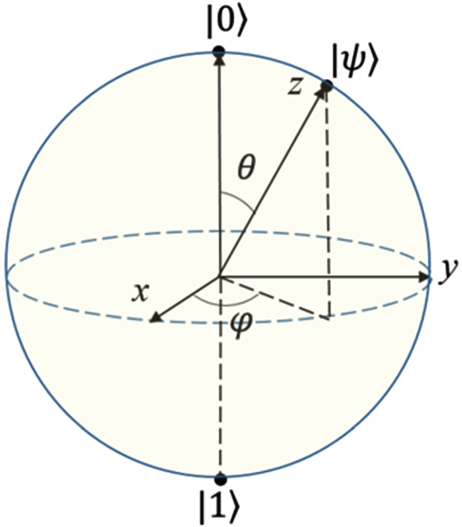
\includegraphics{./images/spin-superpostition.jpg}
    \caption{Spin eines Elektrons in Superposition \cite{noauthor_cpb_27_9_090308_f8jpg_nodate}}
    \label{fig:spin}
\end{figure}

\subsubsection{Quantenverschränkung}



\subsection{Implementierung eines Quantencomputers}


